\documentclass[14pt]{beamer}
\usetheme{Dresden}
\usecolortheme{beaver}

\usepackage{xcolor}
\usepackage{listings}
\usepackage{courier}
\usepackage{graphicx}
\usepackage{amsmath}
\usepackage{algorithm2e}

\definecolor{mGreen}{rgb}{0,0.6,0}
\definecolor{mGray}{rgb}{0.5,0.5,0.5}
\definecolor{mPurple}{rgb}{0.8,0,0.82}
\definecolor{backgroundColour}{rgb}{0.95,0.95,0.92}

\lstdefinestyle{CStyle}{
    backgroundcolor=\color{backgroundColour},   
    commentstyle=\color{mGreen},
    keywordstyle=\color{magenta},
    numberstyle=\tiny\color{mGray},
    stringstyle=\color{mPurple},
    basicstyle=\footnotesize,
    breakatwhitespace=false,         
    breaklines=true,                 
    captionpos=b,                    
    keepspaces=true,                 
    numbers=left,                    
    numbersep=5pt,                  
    showspaces=false,                
    showstringspaces=false,
    showtabs=false,                  
    tabsize=2,
    language=C
}

\lstset{basicstyle=\footnotesize\ttfamily,breaklines=true}
\lstset{framextopmargin=50pt,frame=bottomline}

\title{ENGG1003 - Friday Week 1}
\subtitle{Algorithms and Pseudocode}
\author{Brenton Schulz}
\institute{University of Newcastle}
\date{\today}

\begin{document}
\titlepage

\begin{frame} % Algo defn
\frametitle{Algorithms}
\begin{itemize}
\item Informally, an \textit{algorithm} is a series of steps which accomplishes a task
\item More accurately, the steps (instructions) must:
	\begin{itemize}
		\item Have a strict order
		\item Be unambiguous
		\item Be executable
	\end{itemize}
\item ``Executable" means that the \textit{target platform} is capable of performing that task.
	\begin{itemize}
		\item eg: An industrial welding robot can execute ``move welding tip 1~cm left". A mobile phone can't.
	\end{itemize}
\end{itemize}
\end{frame}

\begin{frame} % Algo communication
\frametitle{Algorithms}
\begin{itemize}
\item An algorithm exists purely as an abstract concept until it is communicated
\item We will use:
	\begin{itemize}
	\item \textit{Pseudocode} to communicate algorithms to ourselve's and other people
	\item The languages C and MATLAB to communicate algorithms to computers
	\end{itemize}
\item Pseudocode can be very formal, as engineers we will only use formal rules if required
	\begin{itemize}
		\item eg: When documenting algorithms for other people
		\item Your own ``working out'' can be anything that helps \textit{you}
	\end{itemize}
\end{itemize}
\end{frame}

\begin{frame}[fragile] % car starting example

\frametitle{Algorithm Example 1}
{\footnotesize
\textbf{Example 1:} Algorithm given to mum to start my car (2015 Toyota Tarago) \\
\textbf{Result:}{The vehicle's engine is idling} \\
\textbf{Initialisation:} stand next to the vehicle, key fob in hand 
\begin{enumerate}
\setlength{\itemsep}{1pt}
  \setlength{\parskip}{0pt}
  \setlength{\parsep}{0pt}
\item Depress the unlock button on the key fob, car will beep twice
\item Place key fob in your pocket
\item Enter the vehicle, sit in the driver's seat
\item Ensure that the gear selector has P engaged
\item Depress the brake pedal
\item Observe that the green LED is lit on the engine start button
\item Press the engine start button
\item If engine is not idling
	\begin{itemize}
		\item Call me
	\end{itemize}
\end{enumerate}
}
\end{frame}

\begin{frame} % Car algo discussion
\frametitle{Example Discussion}
\begin{itemize}
\item The process appears over-explained
	\begin{itemize}
		\item Computers are \textit{really stupid}; get in the habit of over-thinking everything
	\end{itemize}
\item The algorithm contained \textit{flow control}
	\begin{itemize}
		\item The final step (``call me") was \textit{conditional} on the car not starting
	\end{itemize}
\item Lets talk briefly about Boolean logic
\end{itemize}
\end{frame}

\begin{frame} % Boolean Logic
\frametitle{Boolean Logic}
\begin{itemize}
\item Computers don't understand ``maybe''
\item A \textit{condition} on execution must be absolutely \textbf{true} or \textbf{false}
\item Boolean logic (or Boolean algebra) is a field of mathematics which evaluates logical statements as either true or false
\end{itemize}
\end{frame}

\begin{frame}[fragile] % C lstlisting examples
\frametitle{C listing template}
\begin{lstlisting}[style=CStyle]
#include <stdio.h>
int main() {
	printf("Custom lstlisting template\n");
}
\end{lstlisting}

\begin{lstlisting}[language=c]
#include <stdio.h>
int main() {
	printf("default C style\n");
}
\end{lstlisting}
\end{frame}

\begin{frame}
\frametitle{Columns Template}
\begin{columns}
\column{1.5in}
left side
\column{1.5in}
right side
\begin{figure}
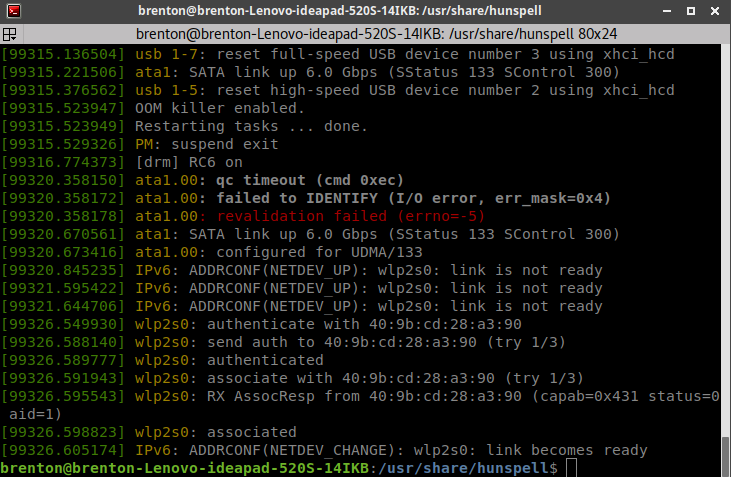
\includegraphics[scale=0.2]{test}
\end{figure}
\end{columns}
\end{frame}


\end{document}
